\documentclass{article}
\usepackage{iclr2027_conference,times}
\usepackage{amsmath,amssymb,amsthm,booktabs,graphicx,microtype,url}
\usepackage[hidelinks]{hyperref}
\newtheorem{proposition}{Proposition}
\newtheorem{corollary}{Corollary}
\newcommand{\E}{\mathbb{E}}
\newcommand{\R}{\mathbb{R}}
\title{Measuring State Aliasing in Neural Multi-Fragment Routing}
\author{Anonymous Authors}
\begin{document}
\maketitle

\begin{abstract}
Flexible construction order changes the information a neural routing decoder
needs. We study a specific interface mismatch: a route decoder reused to join
directed path fragments can observe the same static embeddings, selected-source
context, and feasibility mask in states requiring different optimal endpoints.
We quantify this ambiguity using exact conditional completion costs and the
minimum regret of a policy constrained to share its action across indistinguishable
states. A seven-vertex witness admits a numerically certified positive regret;
controlled paired forests derived from 1,536 larger Euclidean instances exhibit
conflicting optimal decisions in 20.7--29.7\% of pairs across six size/distribution
conditions. We distinguish this constructed stress test from actual policy
occupancy and separate representational limits from optimization failure.
Controlled neural prediction and official-backbone adaptation experiments test
whether making component connectivity observable improves decisions and complete
tours. The study treats paired-endpoint representations and state-abstraction
principles as existing ideas, and evaluates their role in a concrete decoder
transfer failure. Conditional information gains do not, by themselves, establish
an advantage for learned construction order or a stronger routing solver.
\end{abstract}

\section{Introduction}

Neural routing models commonly construct one path by repeatedly selecting its
next vertex. More flexible construction can instead maintain several disjoint
paths and choose which tail to extend. This appears to be a small change to the
action space: select a source, call a pretrained endpoint decoder, and mask
illegal merges. However, a mask answers which actions are feasible, whereas
the value of an action also depends on what those actions leave for the future.
In a path forest, entering a target head commits the solution to traversing
its entire component and leaving through its tail. Two forests can expose the
same legal heads while connecting those heads to different exits.

This paper investigates that discrepancy in adapters around the Attention
Model (AM; \citealt{kool2019attention}) and ICAM
\citep{zhou2026icam}. The claim concerns the observation supplied by our
forest adapters, not the correctness of either native solver. In an archived
limited-budget adaptation study, learned source selection improves on trained
random selection but remains worse than route continuation. That negative
result does not identify its cause: insufficient training, incompatible
representations, and an unhelpful action factorization remain distinct
explanations. We therefore ask a narrower, testable question: \emph{does the
endpoint interface merge states that require different optimal decisions?}

We answer the representational question through exact completion, rather than
teacher likelihood or a heuristic proxy. For an observation class, we compare
the best state-specific actions with the best action shared across its members.
Their difference is a standard conditional Bayes-risk gap. Its use here makes
the missing information measurable and exposes a subtlety in evaluating
counterexamples: the best shared action may be neither state's best action.
We then test information restoration with equal-architecture neural predictors
and controlled residual adapters. Conditional prediction and complete-tour
evaluation are reported separately.

Our contribution is an empirical and implementation-level audit: an exact
diagnostic and certified witness, reproducible observation-matched state
families, and controlled tests of the proposed explanation. Neither paired
endpoint encoding nor path contraction is introduced as a new representation;
DRHG already uses both endpoint coordinates for retained fragments
\citep{li2025drhg}. The resulting evidence must also be interpreted locally.
A source selector can avoid ambiguous states or communicate information through
its source choice. A lower bound for a fixed-source endpoint policy therefore
does not bound the best jointly learned solver.

\section{Directed forests and endpoint observations}
\label{sec:setup}

Let $X=(x_1,\ldots,x_n)$ be Euclidean coordinates with distance $d(u,v)$.
A partial solution $F$ consists of $m$ vertex-disjoint directed paths, including
singletons. Its components have heads $h_i$ and tails $t_i$. Existing directed
edges are fixed: no path reversal, splitting, or reassignment is allowed. With
$m>1$, the action $(i,j)$ joins $t_i$ to $h_j$ for $i\ne j$; the last component
is closed into a tour. We assume a complete graph without capacity, time windows,
or other side constraints.

Given a selected source component $s$, define $Q_F(s,a)$ as the minimum final
tour cost among completions of $F$ containing $t_s\to a$. The one-decision
regret is
\begin{equation}
 r_F(s,a)=Q_F(s,a)-\min_b Q_F(s,b).
\end{equation}
This uses optimal continuation after one decision, not the rollout of an
imperfect downstream model. Fixed internal path costs cancel from regret.

The audited endpoint observation is
\begin{equation}
 z=\phi(X,F,s)=\bigl(E(X),h_s,t_s,M_{F,s}\bigr),
\end{equation}
where $E(X)$ is a static node encoding and $M_{F,s}$ masks illegal heads.
The decoder does not receive all head--tail correspondences, a recurrent
construction history, or the source selector's hidden state. Even an arbitrarily
powerful static encoder cannot recover a dynamic correspondence absent from its
input. This statement would not apply to an encoder recomputed from the forest.
The restriction to the selected source's mask row matters: the full matrix
over all open tails and heads identifies each tail's own component head as
its unique forbidden open head, and therefore reveals their pairing.

\begin{proposition}[Conditional observation regret]
\label{prop:risk}
For a fixed observation $z$, let $\mu_z$ be a distribution over forests with
this observation and common finite action set $A_z$. The smallest expected
regret among policies depending only on $z$ and independent private randomness is
\begin{equation}
 \Delta(z)=\min_{a\in A_z}\E_{\mu_z}Q_F(s,a)
              -\E_{\mu_z}\min_{b\in A_z}Q_F(s,b)
           =\min_{a\in A_z}\E_{\mu_z}r_F(s,a).
 \label{eq:risk}
\end{equation}
For finite support with positive probability on each state, $\Delta(z)=0$
exactly when all statewise optimal-action sets have a common member.
\end{proposition}

\begin{proof}
The expected regret of a randomized policy $p(a\mid z)$ is the convex
combination $\sum_a p(a\mid z)\E_{\mu_z}r_F(s,a)$. Minimizing it selects a
smallest coefficient. Every coefficient is nonnegative, and a coefficient
vanishes exactly when its action has zero regret in every positive-mass state.
\end{proof}

Equation~\eqref{eq:risk} is a finite-action value-of-information identity,
not a new general state-abstraction theorem \citep{li2006abstraction}.
It becomes an operational diagnostic when $Q$ can be computed exactly.
A two-state statistic with access to a sampled pair's identity can be an
optimistic lower bound for a less-informed decoder, rather than its full
distributional Bayes risk. We distinguish these cases in our experiments.

\begin{proposition}[Sufficient component state]
\label{prop:contraction}
For the directed-forest problem above, all future actions, transition costs,
and optimal continuation values are determined by the set of paired endpoints
$\{(h_i,t_i)\}_{i=1}^m$ and the distance function. The remaining optimization
is a directed TSP over components with cost $W_{ij}=d(t_i,h_j)$.
\end{proposition}

Every completion traverses each fixed path contiguously and orders the paths
cyclically. Conversely, every such order is feasible in a complete graph.
Merging $(i,j)$ replaces their pairs by $(h_i,t_j)$ and incurs $d(t_i,h_j)$,
which proves the transition claim. The fixed internal cost is needed only to
recover the total objective. This standard contraction explains the repair;
it does not prove that a particular neural pooling operation preserves all
information. The contracted matrix is generally asymmetric even for symmetric
Euclidean distances. Component means and sizes can aid approximation but are
not necessary for the exact unconstrained continuation problem.

For $m\geq2$, there are $(m-1)!$ directed completion orders and $(m-2)!$ completions after
any legal merge. Every source has $m-1$ legal heads. Source choice alone
therefore does not prune the reachable tour set or select a smaller legal
domain. It may still change learning difficulty and the quality obtained by
an imperfect endpoint policy. A partial-permutation or stabilizer-coset
description does not alter these counts or confer an additional search guarantee.

\section{Exact diagnostics and controlled learning}
\label{sec:experiments}

\subsection{A certified witness}
\label{sec:witness}
Figure~\ref{fig:witness} compares $F_A=\{1\to3,2\to4\}$ with
$F_B=\{1\to4,2\to3\}$ on the same seven vertices and source $0$.
Both forests expose heads $\{1,2,5,6\}$ and the same source context.
The audited AM and ICAM endpoint vectors are exactly identical across the
pair. The optimal heads are $2$ and $5$, respectively. However, the best
\emph{shared} action is head $6$: the regrets are $0.06336798$ and
$0.05438468$, giving $\Delta=0.05887633055$. Using only the two
statewise optimal actions would overestimate the bound.

\begin{figure}[t]
\centering
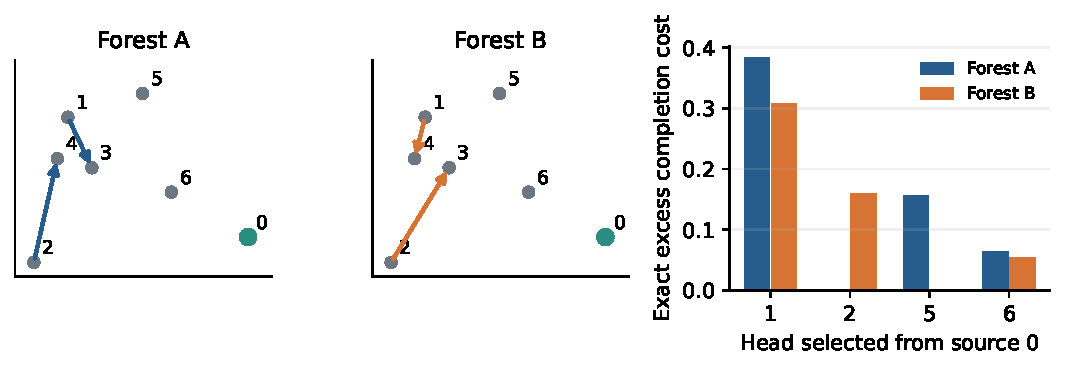
\includegraphics[width=\linewidth]{figures/witness.pdf}
\caption{The selected source (green, vertex 0), legal heads, and static
coordinates are identical. Fixed directed edges (left) change the optimal
conditional completion costs (right). Head 6 is the best compromise for a
decoder unable to distinguish the forests.}
\label{fig:witness}
\end{figure}

An independent enumeration of all $6!=720$ anchored tours reproduces the
24 legal completions of each forest. Interval arithmetic on the recorded
decimal coordinates certifies
$0.058876330550917\leq\Delta\leq0.058876330550931$.
The certificate concerns that specified decimal instance; it makes no
distributional or full-policy claim.

\subsection{Paired fragments from larger instances}
\label{sec:stress}
Before execution, we specified a constructed stress test on 256 fresh geometries in each
of six cells: $n\in\{50,100,200\}$, uniform or clustered sampling. On each
geometry, nearest-neighbor construction followed by at most 100 deterministic
2-opt moves provides a feasible tour. We cut it into six directed paths and
exchange suffixes of two non-source paths. The source path, all component
heads, and the set of tails remain fixed, while two head--tail associations
change. Singleton paths are allowed; only the two swapped paths must have
an internal cut. We enumerate all $5!=120$ cyclic component orders in each
forest and compute Equation~\eqref{eq:risk} under equal pair weights.

\begin{figure}[t]
\centering
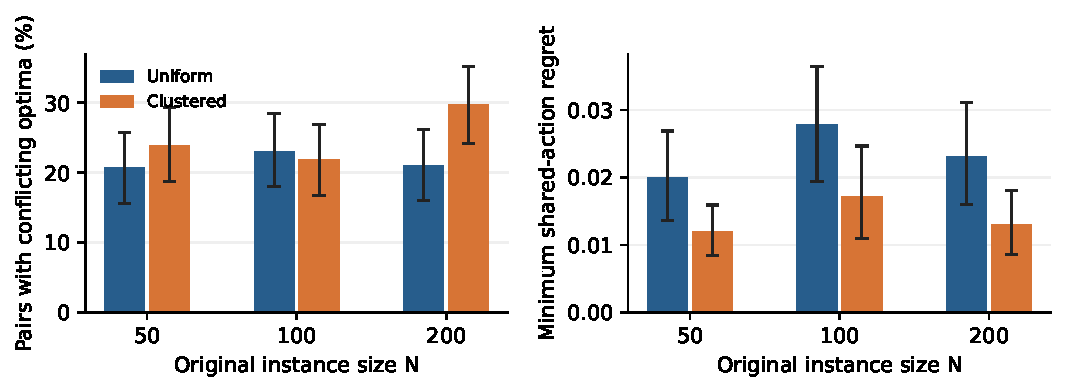
\includegraphics[width=\linewidth]{figures/stress.pdf}
\caption{Constructed counterfactual pairs on larger instances, with six
components per forest. Intervals bootstrap 256 independent geometries per
cell, retaining both states within each unit. The rates describe this generator,
not the occupancy of a deployed neural policy.}
\label{fig:stress}
\end{figure}

\begin{table}[t]
\centering\small
\begin{tabular}{llrrr}
\toprule
Distribution & $N$ & Conflict (\%) & Regret & 95\% CI \\
\midrule
Uniform & 50 & 20.7 & 0.0199 & [0.0136, 0.0269] \\
Uniform & 100 & 23.0 & 0.0278 & [0.0195, 0.0364] \\
Uniform & 200 & 21.1 & 0.0230 & [0.0160, 0.0311] \\
Clustered & 50 & 23.8 & 0.0119 & [0.0084, 0.0159] \\
Clustered & 100 & 21.9 & 0.0172 & [0.0110, 0.0247] \\
Clustered & 200 & 29.7 & 0.0131 & [0.0086, 0.0181] \\
\bottomrule
\end{tabular}

\caption{Exact conditional observation regret on the larger-instance stress
test. Costs use original Euclidean coordinates. Uniform and clustered instances
have different distance scales, so absolute regrets are not a scale-invariant
comparison. An unchanged-pair control has zero regret in all 1,536 cases.}
\label{tab:stress}
\end{table}

Conflicting optimal actions occur in 20.7--29.7\% of pairs
(Table~\ref{tab:stress}). Positive mean regret is not limited to the selected
witness. The construction also exposes a limitation: swapping suffixes can
produce a poor counterfactual forest and does not preserve a policy's visitation
distribution. These figures establish the reach of the interface ambiguity
within a precisely specified family, not its prevalence during ordinary solving.

\subsection{Learning with and without connectivity}
\label{sec:conditional}
We isolate connectivity in a supervised task with exact action values.
Training uses 40,000 independent uniform nine-node geometries, each with two
forests obtained from different matchings of three prescribed heads to three
prescribed tails; the remaining three vertices are singletons, including the
selected source. Validation has 3,000 different geometries. Each test condition
has 4,500 new geometries from three data seeds. Both members of a pair always
remain in the same split. Zero-shot tests vary the node count to 7, 11, and 13
or replace uniform coordinates by three Gaussian clusters.

Blind and aware predictors use the same three-layer, width-128 Transformer
(415,489 parameters), with no positional encoding, and 10,000 AdamW updates
of batch 512. Both receive coordinates relative to the source, head/tail
roles, and singleton/non-singleton indicators. This enriched blind observation
is deliberately more informative than the audited host interface. Only the
aware predictor receives true partner-coordinate displacements. Models
regress exact action regrets; validation regret selects the checkpoint.
Three independent initialization seeds share the data and minibatch streams.
An additional control trains the same network with independent random
pairings, preserving active feature channels without providing true connectivity.

\begin{table}[t]
\centering\small
\begin{tabular}{lrrrrr}
\toprule
Test & Blind & Random pairing & True pairing & Assignment & Nearest \\
\midrule
Uniform 9 & 0.03422 & 0.03374 & 0.00645 & 0.03629 & 0.07744 \\
Clustered 9 & 0.01726 & 0.01778 & 0.00649 & 0.01667 & 0.03354 \\
Uniform 7 & 0.03338 & 0.03502 & 0.00693 & 0.04154 & 0.08148 \\
Uniform 11 & 0.03392 & 0.03389 & 0.01227 & 0.03045 & 0.07081 \\
Uniform 13 & 0.03332 & 0.03295 & 0.01887 & 0.02626 & 0.06704 \\
\bottomrule
\end{tabular}

\caption{Exact fixed-source completion regret, averaged over three training
seeds and paired states. This is not complete-tour solver performance.
The random-pairing control and assignment-relaxation heuristic are supplementary
controls designed after pilot validation. All final selection uses validation.
Every condition has 4,500 independent test geometries.}
\label{tab:conditional}
\end{table}

The true-pairing predictor reduces IID regret from 0.03422 to 0.00645
(81.2\%). The paired absolute reduction is 0.02777, with a geometry-and-seed
bootstrap 95\% interval [0.02572, 0.02981]. The independently trained random-pairing
control obtains 0.03374, close to the blind predictor. Thus active extra input
channels alone do not explain the benefit. Table~\ref{tab:conditional} retains
distribution and size shifts and inexpensive nearest-head and cycle-cover
assignment comparators. The assignment score uses a lower-bound relaxation;
it is not an exact-completion oracle.

\begin{figure}[t]
\centering
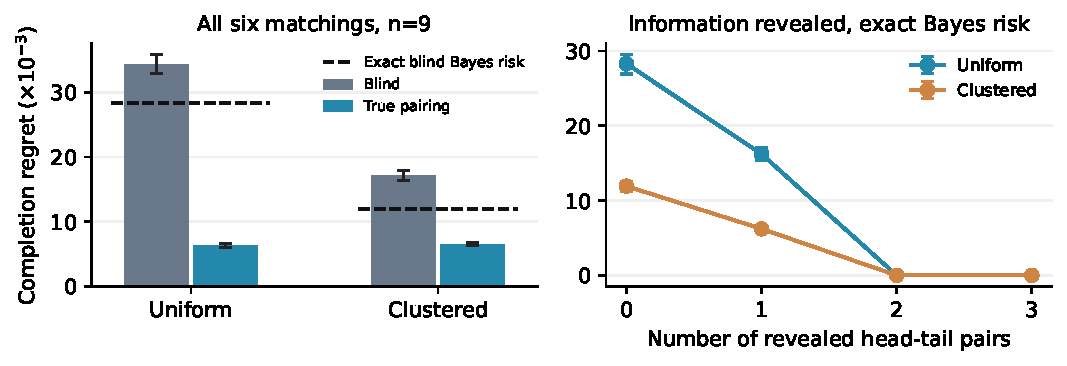
\includegraphics[width=\linewidth]{figures/conditional.pdf}
\caption{A supplementary exhaustive observation-class evaluation on the same
held-out geometries. Left: all $3!=6$ possible matchings, with learned-model
means over three seeds and geometry-bootstrap intervals. Right: reveal the
partners of a predetermined subset of heads and recompute exact Bayes risk.
These curves concern the specified observation family, not native-host occupancy.}
\label{fig:conditional}
\end{figure}

Enumerating all six matchings instead of a sampled pair yields an exact
Bayes risk of 0.02831 for the enriched blind observation on uniform geometries.
The aware model achieves 0.00633 on this same family
(Figure~\ref{fig:conditional}). Revealing one prescribed partner reduces
the risk to 0.01622; revealing two determines the third and reduces it to zero.
This full-family computation avoids confusing a pair-aware oracle with the
Bayes limit for the actual controlled observation.

Swapping the two true associations at test time while keeping model weights
fixed raises IID regret to 0.06271. This is a sensitivity intervention and a
distribution change, not a retrained baseline. Together with the independently
trained random-pairing control, it supports the role of connectivity in the
conditional task. Independent Held--Karp checks of stored labels agree with
enumeration to floating-point precision; coordinate hashes exclude leakage,
blind predictions are exactly identical within each pair, and the largest
measured permutation-equivariance error is $2.98\times10^{-7}$.


\section{From conditional decisions to complete tours}
\label{sec:hosts}

\subsection{Archived adaptation evidence}
We separately audit an existing official-host experiment comprising AM and
ICAM, route continuation, trained random-source forests, and learned-source
forests, with three joint-training seeds per arm. Models receive 2,500
endpoint-supervision updates followed by 300 reinforcement-learning updates;
the three seeds share the relevant warmup. The dataset, trajectory count,
and updates are matched, but training and inference wall times are not.
This is a limited adaptation screen, not evidence of convergence. We recompute
its tables from archived per-instance costs and retain its negative outcomes.

\begin{table}[t]
\centering\small
\begin{tabular}{llrrrr}
\toprule
Host & Test & Route & Random & Learned & Learned excess (\%) \\
\midrule
AM & U200 & 11.5579 & 18.2188 & 14.2735 & 23.50 \\
AM & C200 & 8.0337 & 17.8553 & 11.9997 & 49.37 \\
AM & U500 & 19.7023 & 31.7857 & 24.5729 & 24.72 \\
ICAM & U200 & 10.8307 & 12.6999 & 11.5086 & 6.26 \\
ICAM & C200 & 5.2792 & 8.1126 & 6.4374 & 21.94 \\
ICAM & U500 & 16.9091 & 21.1741 & 18.3969 & 8.80 \\
\bottomrule
\end{tabular}

\caption{Archived adaptation screen, kept separate from new interventions.
U200/C200/U500 denote uniform TSP200, clustered TSP200, and uniform TSP500.
Entries average three joint seeds sharing warmup; lower is better.
Learned excess is relative to adapted route. No inference-time equivalence
or state-repair conclusion follows from this table.}
\label{tab:historical}
\end{table}

Learned source selection beats trained random selection on uniform TSP200,
yet costs remain 23.50\% above route for AM and 6.26\% above route for ICAM
(Table~\ref{tab:historical}). All three predefined size/distribution settings
favor route in mean cost. This motivates diagnosis
but does not show that aliasing caused the entire loss. Nor do 300 updates
establish an upper limit on a method trained to convergence.

Native deployment budget is a separate issue. In an additional archived
evaluation, ICAM with all $n$ starts and eight geometric transformations has
gaps to a feasible LKH reference of 0.27\% on U200, 0.76\% on U500, and
10.62\% on C200. These are not certified optimality gaps. They also cannot
be compared as equal-compute results to a single forest rollout. A weak
single-start baseline can exaggerate practical headroom.

\subsection{Controlled component-state intervention}
\label{sec:repair}
We next test whether the component-state intervention transfers to complete
tours with official AM and ICAM backbones.  For each backbone we compare four
arms---route or uniformly random source selection, each with blind or aware
component inputs---under three independent training seeds.  The residual has
58,306 parameters in every arm.  In the frozen setting only the residual is
trained; in the decoder setting the encoder remains frozen while the native
decoder and residual are adapted.  Each arm receives 12,000 supervised updates
on the same native-plus-2-opt teachers.  Checkpoints are selected by complete
tour validation before four disjoint final-test sets are generated.  No learned
source policy is used in this experiment.

\begin{table}[t]
\centering\scriptsize
\resizebox{\linewidth}{!}{\begin{tabular}{lllrrrrr}
\toprule
Host & Training & Test & Native & Route-B & Route-A & Forest-B & Forest-A \\
\midrule
ICAM & Frozen & U100 & 7.828 & 7.860 & 7.851 & 9.290 & 9.095 \\
ICAM & Frozen & C100 & 4.012 & 3.938 & 3.917 & 5.579 & 5.536 \\
ICAM & Frozen & U200 & 10.837 & 10.871 & 10.861 & 13.397 & 13.209 \\
ICAM & Frozen & C200 & 5.256 & 5.168 & 5.150 & 8.175 & 8.272 \\
\midrule
AM & Frozen & U100 & 8.089 & 8.155 & 8.148 & 11.671 & 11.268 \\
AM & Frozen & C100 & 4.727 & 3.782 & 3.791 & 5.331 & 5.125 \\
AM & Frozen & U200 & 11.621 & 11.600 & 11.563 & 17.323 & 16.877 \\
AM & Frozen & C200 & 7.147 & 5.011 & 4.990 & 8.153 & 7.781 \\
\midrule
ICAM & Decoder & U100 & 7.806 & 7.868 & 7.836 & 9.049 & 9.661 \\
ICAM & Decoder & C100 & 4.074 & 3.946 & 3.959 & 5.143 & 4.731 \\
ICAM & Decoder & U200 & 10.787 & 10.900 & 10.826 & 12.939 & 13.848 \\
ICAM & Decoder & C200 & 5.284 & 5.184 & 5.194 & 7.147 & 6.435 \\
\midrule
AM & Decoder & U100 & 8.077 & 8.178 & 8.139 & 10.851 & 10.493 \\
AM & Decoder & C100 & 4.812 & 3.762 & 3.758 & 4.925 & 4.698 \\
AM & Decoder & U200 & 11.559 & 11.515 & 11.508 & 15.546 & 15.133 \\
AM & Decoder & C200 & 7.269 & 4.980 & 4.958 & 6.943 & 6.620 \\
\bottomrule
\end{tabular}
}
\caption{Complete-tour cost for official-backbone interventions (lower is
better). B/A denote blind/aware component inputs. Forest uses a uniformly
random open source; route continues the current path. Each learned entry is
the mean of three training seeds. Frozen and decoder-adapted suites use
different final-test seeds and are not paired across training phases.}
\label{tab:adapter}
\end{table}

The complete-tour results do not mirror the conditional diagnostic.  With a
frozen AM host, awareness lowers forest cost in all four cells, but aware forest
remains 35--56\% worse than aware route.  Frozen ICAM effects are smaller and
mixed across the four cells.  When the ICAM decoder is also adapted, awareness
reduces teacher-state NLL from 1.183 to 0.539 on U100 and from 1.662 to 0.588 on
U200, yet complete-tour forest cost becomes 7.47\% and 7.44\% worse,
respectively.  It improves clustered C100 and C200 forest tours by 7.53\% and
9.18\%, but still trails aware route by 20--28\%.  Across all 16 host, training,
and test cells in Table~\ref{tab:adapter}, aware forest is worse than aware
route.

Three additional source-action RNG seeds reproduce the broad frozen-host
conclusion and show that the sign of small individual ICAM effects is not
stable.  A target-tail shuffling sensitivity test confirms that fitted models
use the supplied correspondence, but it does not construct an alternative
legal forest and is not a causal estimate.  These outcomes separate two claims:
connectivity is valuable in exact conditional decisions, while this residual,
teacher, and random-source training protocol does not turn that information
into a competitive full-tour forest solver.


\section{Related work}
State abstractions preserve different levels of decision information
\citep{li2006abstraction}. BQ-NCO applies bisimulation quotienting to obtain
reduced constructive problems with optimal-solution guarantees
\citep{drakulic2023bqnco}. Our use of conditional Bayes regret examines an
information-losing adapter in the opposite direction: enlarging construction
freedom while retaining an interface designed for a narrower state family.
It is a diagnostic application of established principles.

Multi-fragment construction is an established routing heuristic
\citep{mamano2019multifragment}, and path contraction is also standard.
DRHG explicitly represents a retained segment using both endpoint coordinates
and learns reconnection \citep{li2025drhg}; this is a direct precedent for our
connectivity intervention. L2C-Insert learns insertion positions
\citep{luo2025insert}, and Learning to Segment identifies stable segments to
reduce repeated search \citep{ouyang2026segment}. We do not claim that flexible
construction, paired endpoints, or compression is novel, and do not present
our limited adapters as stronger solvers than these systems.

Variable-order learning is also established in constraint satisfaction
\citep{song2019ordering}. Order-invariant reinforcement learning randomizes
variable order in black-box optimization \citep{goudet2026order}, while MACSIM
uses multi-action assignments and set-based learning
\citep{luttmann2026macsim}. Such training can address ordering and equivalent
trajectories, but it does not automatically reveal omitted connectivity.
Conversely, adding connectivity does not prove that a learned order is useful.
These are separate hypotheses requiring separate controls.

\section{Discussion and limitations}
The evidence supports testing observation sufficiency before attributing
forest-decoder failures to the optimizer or the usefulness of flexible order.
It does not establish a new group algorithm or a general superiority of
multi-fragment routing. The central remaining question is whether measured
conditional information loss predicts gains on the states a solver actually
visits. Exact small-state supervision, constructed larger-state pairs, and
limited pretrained-host adaptation each answer part of that question.
They are not interchangeable measurements. Strong solver claims require
direct modern baselines, trained ordering controls, independent end-to-end
seeds, and matched inference-time frontiers.

\subsection*{AI use statement}
Generative AI tools assisted with the formulation and proof drafts, experimental
design, code implementation and checking, literature review, result interpretation,
and manuscript and figure preparation. The released artifacts distinguish
executed experiments from analysis and preserve their outputs. This statement
does not assert that independent human verification has already been completed.

\subsection*{Reproducibility statement}
The supplementary code provides deterministic data generators, exact-completion
checks, numerical interval verification, training and evaluation scripts,
per-instance outputs, configurations, and file hashes. Protocols distinguish
archived evidence from new experiments and record budget amendments. Appendix
sections give the assumptions, data generation, and statistical units needed
to interpret these artifacts.

\bibliography{../references}
\bibliographystyle{iclr2027_conference}
\appendix
\section{Assumptions and limits of the regret statement}
The observation-conditioned distribution in Proposition~\ref{prop:risk} is
part of the problem specification. A constructed equal-weight pair yields a
valid risk statement for that pair. If a decoder's true observation class also
contains additional states, then an oracle that is told which pair was sampled
has extra information. Its average pairwise minimum can be smaller than the
minimum achievable by a decoder lacking pair identity. We therefore label
pairwise and full observation-class enumeration separately.

Randomization cannot exploit hidden state unless its random seed is itself
correlated with that state conditional on the observation. Recurrent history,
dynamic encoder inputs, or a source-selector hidden message violate the
interface assumed by the bound. A learned source also changes both the
conditional state distribution and the information conveyed by its selected
index. None of our conditional lower bounds is an impossibility theorem for
joint source--target policies.

If approximate action values satisfy
$|\widehat Q_F(s,a)-Q_F(s,a)|\leq\epsilon$ uniformly, the estimated regret
gap differs from the exact gap by at most $2\epsilon$: each of the two terms
in Equation~\eqref{eq:risk} changes by at most $\epsilon$. Feasible heuristic
completions only upper-bound action values, and usually do not provide such
two-sided error control. A disagreement between heuristic completions alone
does not certify positive irreducible regret.

\section{Contraction and completion counts}
Every completion must retain all fixed directed path edges. Contract each path
to a component with its ordered head and tail. A completed tour corresponds to
a cyclic ordering of the $m$ distinguishable components, with one connector
from each component's tail to the next component's head. Conversely any
cyclic component order expands into a Hamiltonian tour because the graph is
complete. Fixing one component to remove rotational duplicates gives
$(m-1)!$ completions. Specifying a legal connector merges two components and
leaves $(m-2)!$ orders. With one component only its closure remains.

Any optimal completion assigns a successor to every open source, so fixing
which source is queried first does not change the optimal completion value
provided all its legal heads remain available. It can nevertheless change
the outcome of a restricted neural policy. These statements concern the
directed fixed-fragment problem. Reversing a fragment changes its fixed
successor assignments; destroy-and-repair, sparse graphs, capacity constraints,
and time windows require different transition and feasibility analyses.

\section{Numerically certified witness}
The witness uses the following recorded decimal coordinates, with zero-based
vertex numbering:
\begin{center}\small
\begin{tabular}{rrr}\toprule
Vertex & $x$ & $y$\\\midrule
0 & 0.9667947888374329 & 0.144645094871521\\
1 & 0.16519033908843994 & 0.6777374148368835\\
2 & 0.01400136947631836 & 0.032273709774017334\\
3 & 0.27172255516052246 & 0.45283347368240356\\
4 & 0.11830371618270874 & 0.4929446578025818\\
5 & 0.49647223949432373 & 0.7829722166061401\\
6 & 0.6254234313964844 & 0.34477776288986206\\\bottomrule
\end{tabular}\end{center}
Each decimal is interpreted as an exact rational. For every squared distance
$q$, integer square roots bound $\sqrt q$ between adjacent multiples of
$10^{-15}$. Summing the lower and upper edge bounds along all anchored tours
and taking actionwise minima bounds each conditional optimal completion cost.
For $L_s(a)\leq Q_s(a)\leq U_s(a)$, a valid lower bound on the equal-pair
regret is
\[
\frac12\min_a\sum_s L_s(a)-\frac12\sum_s\min_a U_s(a),
\]
with the upper bound obtained by interchanging $L$ and $U$.
The verification uses only Python's standard library and checks all 720 tours.
This is a certificate for the specified decimal instance, distinct from
claiming exact real arithmetic on unspecified binary-coordinate inputs.

\section{Larger-instance stress generator}
Uniform instances sample $n$ coordinates independently in $[0,1]^2$.
Clustered instances sample four centers uniformly in $[0.15,0.85]^2$, assign
each vertex uniformly to a center, add independent Gaussian noise with
standard deviation $0.04$, and clip to the unit square. There are 256
geometries per size/distribution cell and no test-dependent selection.
Seeds are $91972000+10n+b$, where $b=0$ for uniform and $b=1$ for clustered.

A nearest-neighbor tour begins at vertex zero. Deterministic best-improvement
2-opt accepts at most 100 improving moves. This is a feasible construction,
not an optimality certificate or a benchmark competitor. Five cut positions
are sampled without replacement among the $n-1$ gaps in its linearized order,
giving six paths. If fewer than two non-source paths have length at least two,
cuts are resampled. From eligible paths, two are sampled and cut internally;
their suffixes are exchanged. The source is the tail of path zero and is
unchanged. All path heads and the set of tails remain unchanged.

For each pair, all 120 directed cycles on six components are enumerated.
Q-values include fixed internal lengths, but these cancel separately within
each forest when computing regret. Both forests are retained, including all
zero-regret pairs. A control duplicating the original forest must yield zero.
In floating-point summaries, a pair is marked conflicting when its minimum
shared-action regret exceeds $10^{-9}$.
Bootstrap intervals use 4,000 resamples of whole geometries, never treating
the two forests as independent observations. These sampling rules are
deliberately explicit because different fragment and counterfactual generators
can give different conflict rates.

\section{Controlled neural prediction protocol}
For $n=2k+3$ vertices, vertex zero is the selected singleton source;
vertices $1,\ldots,k$ are nontrivial component heads and vertices
$k+1,\ldots,2k$ are their tails. The last two vertices are singletons.
An initial uniform random matching defines $k$ length-two components;
swapping two randomly selected matches constructs the second forest.
Coordinates are sampled independently of the matching. The number of
components is $k+3$, so enumerating anchored component cycles is tractable
for the tested $k=2,3,4,5$. Distances and action values are computed in
float64 from coordinates stored as float32.

The shared node features are source-relative coordinates, a head indicator,
a non-head indicator, a source indicator, and a non-singleton indicator.
Two additional channels contain displacement to the paired endpoint in the
aware condition and zeros in the blind condition. Both heads and tails
receive the displacement. There are no positional embeddings. The network
uses an eight-dimensional input projection to width 128, three pre-norm
Transformer layers with eight heads and feed-forward width 256, GELU
activation, and zero dropout. A shared normalized MLP outputs one scalar
per candidate head. Mean-squared error to exact regret trains the scores;
the chosen action minimizes the predicted score over legal heads.

AdamW uses learning rate $3\times10^{-4}$, weight decay $10^{-5}$,
gradient-norm clipping at one, and batch size 512 for 10,000 updates.
Validation runs at the first update and every 500 updates thereafter;
the lowest mean exact validation regret selects the checkpoint. The seeds
are 19091941, 19091942, and 19091943. Train and validation geometry seeds
are 190919101 and 190919201; each test condition concatenates 1,500
geometries from each of seeds 190919301--190919303. The clustered condition
uses three centers in $[0.15,0.85]^2$, Gaussian noise of standard deviation
0.06, and clipping to the unit square. All train, validation, and test
geometries remain disjoint; reusing a data seed at another size does not
create an identical geometry.

The independently trained random-pairing control resamples a uniform matching
for every training example on every update using a separate RNG. It retains
all roles and active feature channels but makes the displayed matching
independent of the label-generating matching. Validation and test use fixed
independent corruption streams. Test-time wrong pairing instead exchanges
the two members' true associations while keeping the aware model fixed.
These two experiments answer different questions. Both are supplementary
mechanism controls designed after initial pilot validation; neither selects
the main predictors using the final test.

The supplementary full-family evaluation holds geometry and roles fixed
and enumerates all six matchings for $k=3$. It therefore computes the exact
Bayes regret for the enriched blind observation and the specified uniform
matching prior. Progressive revelation groups the six matchings by the
partners of heads $1,\ldots,r$ and averages each group's optimal shared
action with its probability. With two known partners the third is determined.
No learned predictor or test-based selection is needed for this calculation.

Statistical summaries first average both paired states within each geometry.
Model means then average three training seeds. Geometry-only intervals
condition on these trained models; additional crossed bootstrap intervals
resample both whole geometries and the three seeds. The latter do not
compensate for having only three training seeds. The assignment comparator
forces each candidate first action and scores an assignment relaxation of
the remaining directed component problem, without requiring a single cycle.
Its lower-bound scores are used as a heuristic ranking, not as exact Q-values.

\section{Archived host study details}
The earlier study starts from the official AM TSP100 epoch-99 checkpoint and
the official ICAM checkpoint. Each host supplies greedy tours for 2,048
uniform TSP200 training geometries, improved by up to 200 best-improvement
2-opt moves. Route and random-order endpoint warmup use 2,500 updates of
batch 32 at learning rate $10^{-5}$; the selected warmup is shared across
the three subsequent joint seeds 1234, 2468, and 4321. The joint stage has
300 updates with four independent instances and four stochastic trajectories
per instance, leave-one-out REINFORCE baselines, host learning rate $10^{-5}$,
selector learning rate $10^{-4}$, and gradient clipping at one.

Joint validation uses 64 instances every 50 updates, including the initial
checkpoint. The primary test has 256 uniform TSP200 instances; secondary
tests have 64 clustered TSP200 and 64 uniform TSP500 instances. The reported
seed uncertainty is conditional on shared warmup. Random source actions use
a documented fixed evaluation RNG; their variation across multiple action
seeds was not estimated in that archived study. Both hosts were evaluated
on the same predefined conditions; failing cells were retained.

The earlier prototype computes endpoint distributions for all sources at
every step. Its forest rollouts are slower than native route construction.
The results are matched by samples and updates, not GPU seconds. The original
source selector uses detached endpoint-probability summaries; its gradient
does not include derivatives through those summaries into the host. These
details limit conclusions about efficiency and optimization.

\section{Artifact organization and research boundaries}
The root protocol distinguishes four work packages: exact controlled learning,
official-host representation intervention, larger-instance counterfactual
stress testing, and theory/literature verification. Analysis scripts regenerate
tables and figures from machine-readable results. Historical cost vectors are
identified by content hashes and are not relabeled as new measurements.

The manuscript provides no claim of a new group-theoretic pruning algorithm,
no guarantee for arbitrary constrained routing, and no equal-time solver
ranking. Full-source freedom and complete-tour reachability concern the
action space, not a deterministic neural policy's actual support. More
training, a learned source policy, an alternative loss, and additional
decoding starts are different interventions and must be compared explicitly.

\end{document}
